%-*- coding: utf-8 -*-   
\documentclass[11pt,a4paper,a4wide,headsepline,bibtotoc,twoside]{scrbook}

\usepackage[T1]{fontenc}
\usepackage{ucs}
\usepackage[utf8x]{inputenc} 
\usepackage{lmodern}
%\usepackage{textcomp}
\usepackage{garamond}
\usepackage{helvet}
\usepackage{courier} % used to display code
\usepackage{color}
 \usepackage{anysize}
\marginsize{3cm}{2cm}{1cm}{1cm}
\textwidth 15 cm 

\definecolor{rltblue}{rgb}{0.1,0.1,1}


\usepackage{listings}
\lstset{ %
  language=SQL,                % the language of the code
  basicstyle=\ttfamily,           % the size of the fonts that are used for the code
  numbers=left,                   % where to put the line-numbers
  numberstyle=\footnotesize,          % the size of the fonts that are used for the line-numbers
  stepnumber=2,                   % the step between two line-numbers. If it's 1, each line 
                                  % will be numbered
  numbersep=5pt,                  % how far the line-numbers are from the code
  backgroundcolor=\color{white},      % choose the background color. You must add \usepackage{color}
  showspaces=false,               % show spaces adding particular underscores
  showstringspaces=false,         % underline spaces within strings
  showtabs=false,                 % show tabs within strings adding particular underscores
  frame=single,                   % adds a frame around the code
  tabsize=2,                      % sets default tabsize to 2 spaces
  captionpos=b,                   % sets the caption-position to
                                % bottom 
  breaklines=true,                % sets automatic line breaking
  breakatwhitespace=false,        % sets if automatic breaks should only happen at whitespace
  title=\lstname,                   % show the filename of files included with \lstinputlisting;
                                  % also try caption instead of title
  numberstyle=\tiny\color{gray},        % line number style
  keywordstyle=\color{blue},          % keyword style
  columns=fixed,
  commentstyle=\color{dkgreen},       % comment style
  stringstyle=\color{mauve},         % string literal style
  escapeinside={\%*}{*)},            % if you want to add a comment within your code
  morekeywords={*,...}               % if you want to add more keywords to the set
} 
\usepackage[dvips]{thumbpdf}
\usepackage[pdftex,
colorlinks=true,
urlcolor=rltblue,               % \href{...}{...}
anchorcolor=rltbrightblue,
filecolor=rltgreen,             % \href*{...}
linkcolor=rltblue,               % \ref{...} and \pageref{...}
menucolor=webdarkblue,
citecolor=webbrightgreen,
pdftitle={Projecto de Fim de Curso},
pdfauthor={Pedro Moreira, 10015},
pdfsubject={Agrometeo Alentejo},
pdfkeywords={Estação meteorológica, agricultura, worpress},
% pdfadjustspacing=1,
pagebackref=false,
pdfpagemode=None,
bookmarksopen=true]{hyperref}
\pdfcompresslevel=9

\usepackage[pdftex]{graphicx}
\usepackage{thumbpdf}

%%%%%%%%%%%%%%%%%%%%%%%%%

%% escrita em portugues
%\usepackage[latin1]{inputenc}
\usepackage[portuges]{babel}

% virgulas numericas correctas
\usepackage{icomma}

% processamento com indicação de linhas pelo pacote xdvi
\usepackage{srcltx}

\bibliographystyle{plain}

%% introducao do ambiente de geracao de indices
\usepackage{makeidx}

\usepackage[isu,small,ruled]{caption}
\setlength{\captionmargin}{0.5cm}
\usepackage{prettyref}

%\usepackage[portuges]{minitoc}

%% pacotes matematicos AMS
\usepackage[intlimits]{amsmath}
\usepackage{amssymb}

% simbolos matematicos
%\usepackage{jeffe}
%% graficos com dvips
%%
%%
%%
%% as fontes para os graficos são de 12pt, helvetica
% \usepackage[dvips]{graphics}
\usepackage{lscape}
\usepackage{subfigure}

% captions
\usepackage{float}
\usepackage{rotating}

%% bibliografia por temas e capitulos
%\usepackage{bibtopic}

%% especificacoes para portugues
\newrefformat{teorema}{Teorema~\ref{#1}}
\newrefformat{cha}{Cap{\'\i}tulo~\ref{#1}}
\newrefformat{sec}{Sec{\c c}{\~a}o~\ref{#1}}
\newrefformat{tab}{Tab.~\ref{#1}}
\newrefformat{eq}{Eq.~\ref{#1}}
\newrefformat{def}{Def.~\ref{#1}}
%% na p{\'a}g. #2}
\newrefformat{fig}{Fig.~\ref{#1}}
%% na p{\'a}g. #2}
\newrefformat{alg}{Alg.~\ref{#1}}
%%\newrefformat{pag}{P{\'a}g.~\ref{#1}}

\newtheorem{assuncao}{Assun{\c c}{\~a}o}
\newtheorem{definicao}{Defini{\c c}{\~a}o}
\newtheorem{teorema}{Teorema}

\newcommand{\goodgap}{%
\hspace{\subfigtopskip}%
\hspace{\subfigbottomskip}}

\newcommand\glossaryname{Gloss{\'a}rio}

% processamento mais agradável de figuras
\renewcommand{\topfraction}{0.85}
\renewcommand{\textfraction}{0.1}
\renewcommand{\floatpagefraction}{0.75}

%%% fontes para cabecalhos e inicios de capitulos
%%% \renewcommand{\sectfont}{\rmfamily\bfseries}

%\renewcommand{\headfont}{\scshape}

 \renewcommand*\contentsname{Índice Geral}


%%
\usepackage{supertabular}

% posicionamento arbitrario de texto
\usepackage[absolute]{textpos}
\usepackage{type1cm}
\usepackage{lettrine}
\usepackage{multind}
\makeindex{aut}
\makeindex{alf}

\begin{document}

\garamond
%% modos de armazenamento de imagens em Postscript encapsulado
%% e comprimido
\DeclareGraphicsRule{eps.gz}{eps}{eps.bb}{`gunzip -c #1}
%% directoria onde se armazena os ficheiros
\graphicspath{{EPS/}}

\frontmatter
%\maketitle
\thispagestyle{empty}
\begin{titlepage}
  \vspace*{2cm}
  \baselineskip=24pt

\fontshape{bold}
\fontsize{20}{30}
  \textblockorigin{0cm}{0cm}
  \begin{textblock*}{16cm}(2.5cm,2.5cm)
    \centering
    \textbf{{INSTITUTO POLITÉCNICO DE BEJA
  \end{textblock*}

   \textblockorigin{0cm}{3cm}
   \begin{textblock*}{16cm}(2.5cm,3cm)
     \centering
\fontshape{bold}	
\fontsize{24}{30}
       \textbf{{Projecto de Fim de Curso
\end{textblock*}




   \textblockorigin{0cm}{3cm}
	\centering
   \begin{textblock*}{15cm}(3cm,8cm)
     \centering
      
 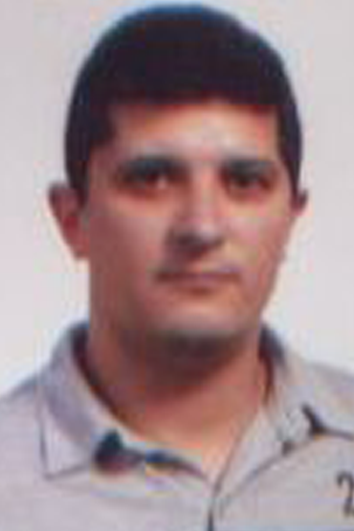
\includegraphics[width=3cm]{pedro.png}
	
   \end{textblock*}


   \textblockorigin{0cm}{5cm}
   \begin{textblock*}{16cm}(2.5cm,13cm)
     \centering
\fontshape{bold}	
\fontsize{16}{16}
       \textbf{{Pedro Miguel Clemente Dias Moreira\\}}
   \end{textblock*}
   \textblockorigin{0cm}{5cm}
   \begin{textblock*}{16cm}(2.5cm,14cm)
     \centering
\fontshape{bold}	
\fontsize{16}{16}
       \textbf{{n.º 10015\\}}
   \end{textblock*}


   \textblockorigin{0cm}{5cm}
   \begin{textblock*}{16cm}(2.5cm,21.2cm)
     \centering
\fontshape{bold}	
\fontsize{12}{20}
       \textbf{17 de março 2012}
   \end{textblock*}
   
\end{titlepage}
%%
%% capa.tex
%% 
%% Made by Pedro Moreira
%% Email   <mail@pedromoreira.org>
%% 
%% Started on  Sun Jun 17 01:17:00 2012 Pedro Moreira
%% Last update Sun Jun 17 23:50:33 2012 Pedro Moreira
%%

\thispagestyle{empty}
\cleardoublepage

\mainmatter


\cleardoublepage
\pagestyle{headings}
\setcounter{page}{1}
\pagenumbering{arabic}
\tableofcontents
\cleardoublepage

%%\part{}

\chapter{Introdução}
A previsão meteorológica é importantíssima para a tomada de decisões no âmbito da agricultura. Com ela é possível melhorar a caracterização dos acidentes meteorológicos com maior risco para as culturas em causa. 
Com a cada vez maior inconstantibilidade do tempo, torna-se fulcral ter uma melhor capacidade de prever as condições meteorológicas para uma melhorar a preparação contra acidentes meteorológicos.
\\Para se conseguir uma previsão mais correcta, é muito importante ter uma quantidade considerável de dados observadoos para diminuir a margem de erro das mesas. Uma das formas para se obter mais dados observados, será a utilização de estações meteorológicas em mais locais do território português.
\\Com esta oportunidade da parceria com a FAABA e o IM torna-se mais simplificada esta tarefa.
 

\section{Objectivos}
Este projecto pretende criar uma solução que sirva de ponte entre os agricultores do Baixo Alentejo e o Instituto de Meteorologia para que se possa apresentar as previsões meteoreológicas, avisos e alertas aos agricultores para lhes facilitar o processo de decisão no que concerne à sua actividade.

\section{Estrutura do Relatório}
Neste trabalho é apresentada uma solução para implementação de estações metereológicas, a recolha dos respectivos dados, armazenamento e envio ao Instituto de Meteorologia.
Na segunda parte do trabalho é apresentada a forma como obtemos as previsões meteorológicas e climatologia calculados pelo IM.
Por fim é apresentada a interface criada para a aplicação que apresentará aos utilizadores não só os dados observados por cada uma das estações, mas também as previsões calculadas pelo IM.
\chapter{Recolha de Dados}
	As estações metereológicas estarão localizadas dispersamente 
	o que torna mais complicada a tarefa da recolha automática dos dados das mesmas.
	
	\\Como existem vários tipos de estações metereológicas que, dependendo do fabricante, 
	terão diferentes formas de acesso aos dados, o sistema deverá estar preparado para 
	acolher equipamentos com as mais variadas formas de acesso aos dados.

	\\De acordo com os dados fornecidos pela FAABA, e partindo do princípio que 
	os equipamentos utilizados pelos seus membros serão uniformes no que diz respeito 
	a marca, apresentamos uma solução com equipamentos da marca adcon.


\section{Estado da Arte}
Existem vários avanços em sistemas deste género a nível mundial. 
\\Em Portugal, mais especificamente no Algarve, existe uma rede de estações meteorológicas, que além de fornecer os dados aos agricultores, permite às escolas um estudo mais aprofundado dos dados e, através dos seus laboratórios, estudar os resultados e chegar a conclusões acerca dos mais variados tipos de problemas. 
\\Nos Estados Unidos, mais concretamente no estado de Washington foi criado um sistema autónomo de raiz que liberta os agricultores das marcas e equipamentos existentes no mercado, tornando as soluções mais baratas e permitindo uma maior contribuição e evolução das escolas na área. É de notar uma enorme vantagem na utilização do paradigma das redes de sensores wireless, que tornam muito mais simples e barata a resolução dos problemas de comunicação entre os vários equipamentos. 


\section{Requisitos Funcionais}
Estações meteorológicas da marca adcon, apetrechadas com equipamentos para comunicações, mais concretamente utilizando UHF e nos casos de estações fora do alcance terão que ter equipamentos para comunicação GSM / GPRS. Esta marca tem uma enorme vantagem pois utiliza o paradigma das redes de sensores wireless.
Para a comunicação com as estações e armazenamento dos dados, deverá existir um gateway também da marca adcon.

	\subsection{Estações Meteorológicas}
	As estações devarão ter vários sensores, nomeadamente temperatura, medição da velicidade e direcção do vento, humidade, pluviosidade e pressão atmosférica.
	Todas elas deverão estar equipadas com material de comunicação.

	\\As estações deverão ter equipamento de rede instalado, sendo que nos caso de existir dificuldade de comunicação numa estação deverá ser estudada a aplicação de um aparelho GPRS na mesma, ou em uma próxima, para servir de repetidor e fazer a ligação entre outras que também tenham dificuldades de comunicação.
	\subsection{Gateway}
	É necessario pelo menos um gateway da marca adcon para a conexão às várias estações, este gateway, além de controlar todas as comunicações tem a capacidade de armazenar dados localmente e disponibilizá-los através de um serviço http.
\\Por esta via é depois possivel o tratamento dos mesmo para troca de informação com o Instituto de Meteorologia, bem como o seu armazenamento no servidor web para a apresentação dos dados no interface disponível ao público.

	\subsection{Servidor}
	É necessario um servidor que tenha instalado o Apache, mysql e php. Nele será instalado um portal wordpress que será o principal interface para a disponibilização da informação ao público.


\section{Requisitos Não Funcionais}
	\subsection{Conectividade}
	É necessário que exista uma elevada taxa de conectividade entre todas as estações e o gateway. Assim, deveráser efectuada uma medição das ligações periodicamente para a avaliação das condições de ligação para se ponderar a colocação de eventuais pontos de acesso ou intalação de aparelhos GPRS nas estações com mais dificuldade de acesso.
\\É tambem necessária uma boa manutenção dos equipamentos e sua substituição em caso de mau funcionamento.

	\subsection{Segurança}
	As estações deverão estar protegidas de acessos indevidos. O acesso aos dados do gateway deverá ser limitado ao menor número de utilizadores possível or forma a evitar congestionamento no seu acesso. 

	\subsection{Desempenho}
	O servidor deverá ser capaz de lidar com múltiplos acessos e aceder a um elevado número de estações. 
\\ Deverão existir formas de evitar quebras dos serviços ou reposição dos mesmo em caso de eventuais falhas.
\chapter{Troca de Dados com o Instituto de Meteorologia}
Os dados recolhidos deverão ser facultados ao Instituto de Meteorologia, para poder elaborar as previsões através dos seus algoritmos e com a ajuda dos dados recolhidos de outras estações.

\section{Restrições}

\section{Requisitos Funcionais}
Ainda falta obter os requisitos para se efecutar esta operação.

\section{Requisitos Não Funcionais}

\chapter{Interface Gráfica}
\section{Problema}
\section{Estado da Arte}
Apresentação da tendência na apresentação das interfaces gráficas.

\section{Restrições}
A interface deverá ser elaborada na plataforma wordpress.

\section{Requisitos Funcionais}
Deverá ser implementada uma base de dados em mySQL.


\section{Requisitos Não Funcionais}
A interface deverá respeitar as regras de acessibilidade W3E (AA no mínimo).

\chapter{Conclusão}
\chapter{Trabalho Futuro}
\bibliography{bibliografia}
\end{document}